\documentclass[a4paper]{article}

%% Language and font encodings
\usepackage[english]{babel}
\usepackage[utf8x]{inputenc}
\usepackage[T1]{fontenc}


%% Sets page size and margins
\usepackage[a4paper,top=3cm,bottom=2cm,left=3cm,right=3cm,marginparwidth=1.75cm]{geometry}

%% Useful packages
\usepackage{amsmath}
\usepackage{graphicx}
\usepackage{mathptmx}
\usepackage{float}
\usepackage{lmodern} % math, rm, ss, tt
\usepackage[T1]{fontenc}
\usepackage[colorinlistoftodos]{todonotes}
\usepackage[colorlinks=true, allcolors=blue]{hyperref}

\title{Montel for ID20}
\author{Aouadi Yiones}

\begin{document}
\maketitle


\begin{figure}[H]
\centering
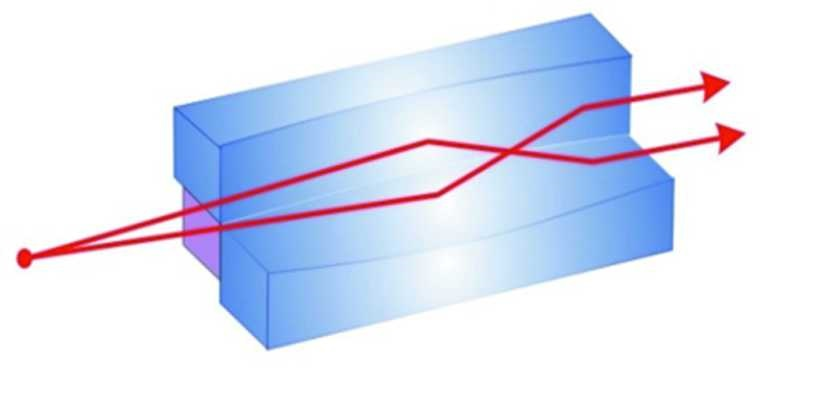
\includegraphics[width=1\textwidth]{Montel.jpg}
\end{figure}

\section{Introduction}
With the following document I want to report the reuslts obtained in the simulation of a beam through a Montel system (optical system composed bye two orthogonal mirro). It has been studied the tolerance in orthogonality using the parameter similar tho those distribuited by the AXO DRESDEN Gmbh \cite{greenwade93}

\section{System}

In this simulation was used a Monte-Carlo approach with the following specification

\subsection{Source}

Source parameters
\begin{itemize}
\item Number of rays: $10^6$
\item Source size: 1*1 $\mu $$m^2$
\item Divergence: gaussian profile with a FWHM OF 75$\mu $$rad$ ($\sigma $ = 10.6 $\mu $$rad$)
\end{itemize}
Figure \ref{fig:beam at the source} show the source geometry, and figure \ref{fig:source divergence} show the divergence of the source beam

\begin{figure}[H]
\centering
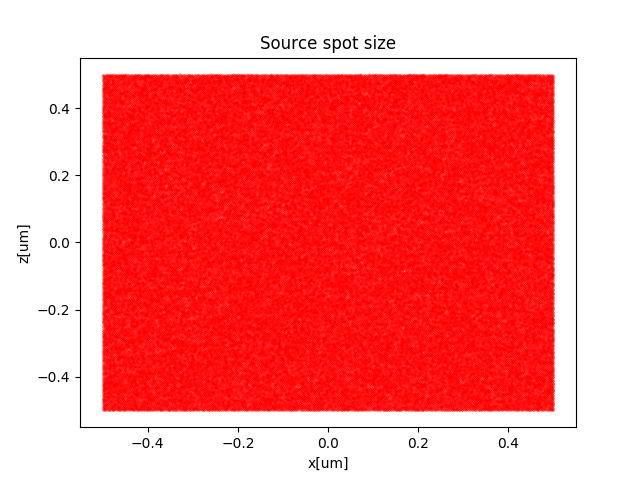
\includegraphics[width=0.6\textwidth]{Spot.png}
\caption{\label{fig:beam at the source}Source size 1*1 $\mu $$m^2$ }
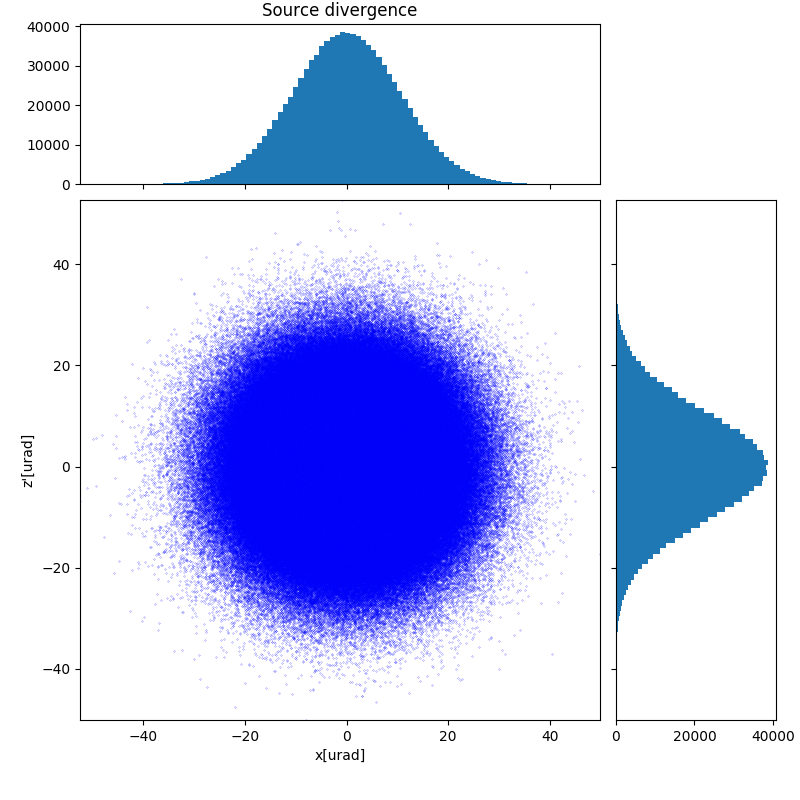
\includegraphics[width=0.8\textwidth]{Initial_divergence.png}
\caption{\label{fig:source divergence} Beam source}
\end{figure}


\subsection{Montel system}

As mentioned before, two orthogonal mirror (parabolic in this case) were used, with parameters
\begin{itemize}
\item Focal distance (distance between the source and the center of the mirror): f=351$mm$
\item Mirror length: L=300$mm$
\item Mirror width:  W=100$mm$
\item $\Delta$ (error max. between the orthogonal configuration of the two mirrors, negative correspond to have the mirror closer each other, positive further):      $\Delta$ = $\pm$0.03$^{\circ}$
\item Parabola parameter: p=0.23$mm$, that correspond to an incidence angle of 18.1$mrad$ (see appendix A)
\end{itemize}

In figure \ref{fig:Montel system} is showed a graphic simulation on the Montel system with the parameter used. As show the source is positioned in a place such that it hit the center of the system with the correct angle


\begin{figure}[H]
\centering
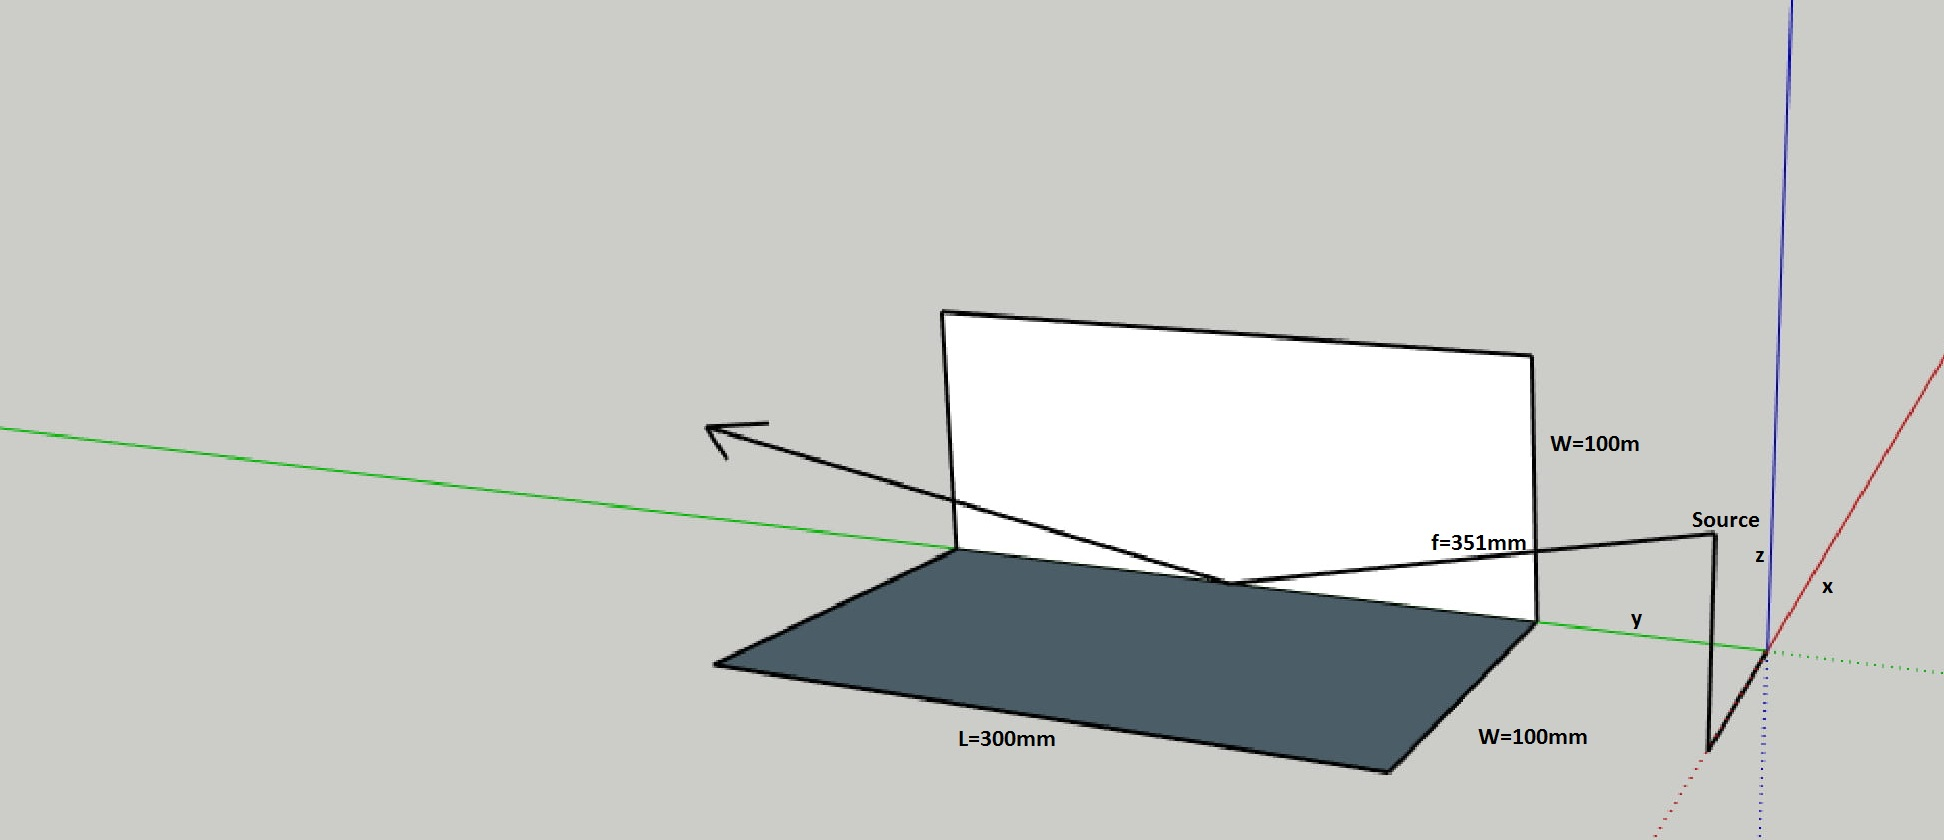
\includegraphics[width=1\textwidth]{MontelSystem.jpg}
\caption{\label{fig:Montel system} Montel system}
\end{figure}
\section{Results of beam figure and footprint}

The image plane is positioned at 0.65m from the center of the Montel system. The property of the beam at the image plane are showed in figure \ref{fig:image}, it is obtained a new spot size with a length of 60$\mu$$m$ in the x direction and 100$\mu$$m$ in the z direction, and the divergence has a FWHM of 40$\mu$$rad$


\begin{figure}[H]
\centering
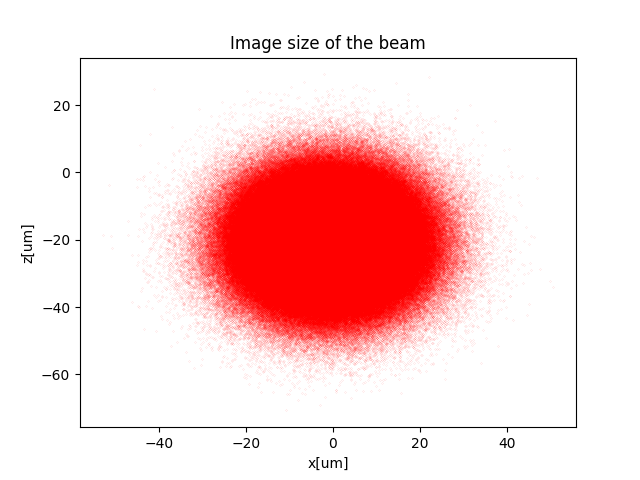
\includegraphics[width=0.495\textwidth]{image_spot.png}
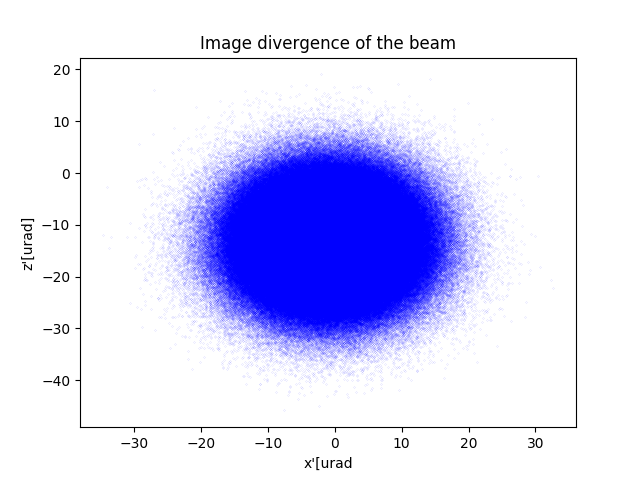
\includegraphics[width=0.495\textwidth]{image_divergence.png}
\caption{\label{fig:image} footprint, on the xy-mirror (left figure), zy-mirror (right figure). The red dots are those ray that hit before xy-mirror and after zy-mirror, the blue ones before xy-mirror and after zy-mirror}
\end{figure}


Moreover is interesting to note the footprint of the two mirror (figure \ref{fig:footprint_oe1}) that, this footprint is interesting because the area hit have a greater component on the y direction (because the beam is grazing), than in the other direction, in fact the x-length of the xy-mirror, and the z-length of the zy-mirror, is very small (at the order of 20$\mu $$m$), on the contrary the y-length is huge $\simeq $ 200$mm$

\begin{figure}[H]
\centering
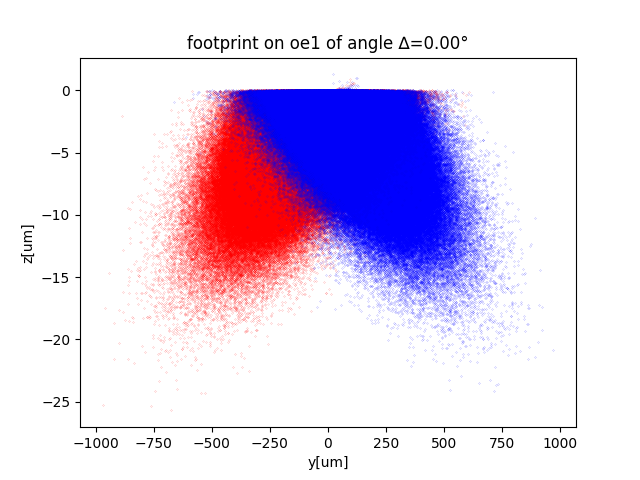
\includegraphics[width=0.495\textwidth]{footprint_oe1.png}
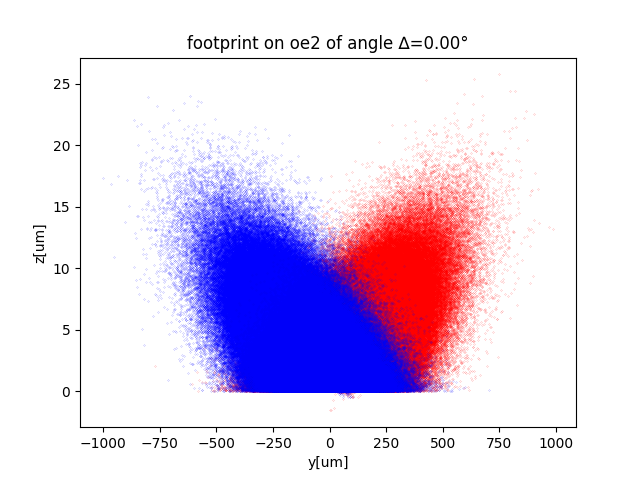
\includegraphics[width=0.495\textwidth]{footprint_oe2.png}
\caption{\label{fig:footprint_oe1} footprint, on the xy-mirror (left figure), zy-mirror (right figure). The red dots are those ray that hit before xy-mirror and after zy-mirror, the blue ones before xy-mirror and after zy-mirror}
\end{figure}



\section{Analysis of orthogonality}
Figure \ref{fig:histogram} it presents the interesting histograms versus the horizontal anlge x' when the angle between the mirrors change ($\alpha $ = 90$^\circ$ + $\Delta$). It can be noted a improvement of the collimation of the beam changing the angle in the case of closer mirrors (delta=-0.01 degree) but.
\newline Figure \ref{fig:FWHM} show the trend of the FWHM of the x' changing the angle $\Delta$, it is possible to note a minimum for negative angle (this ideal situation is the pink curve reported in figure \ref{fig:histogram}) after that the situation become worse, moreover, the behavior of the FWHM is not symmetrical with respect to 0$^\circ$, in case of positive angle the beam behave worse with respect to the orthogonal situation

\begin{figure}[H]
\centering
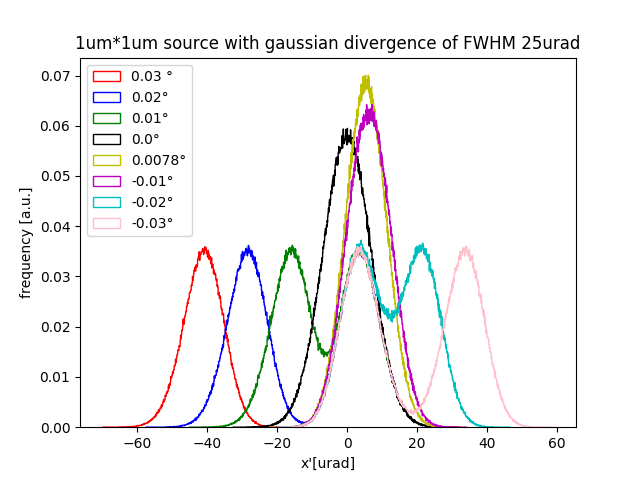
\includegraphics[width=0.8\textwidth]{histogram.png}
\caption{\label{fig:histogram} x' values after the Montel system}
\end{figure}

\begin{figure}[H]
\centering
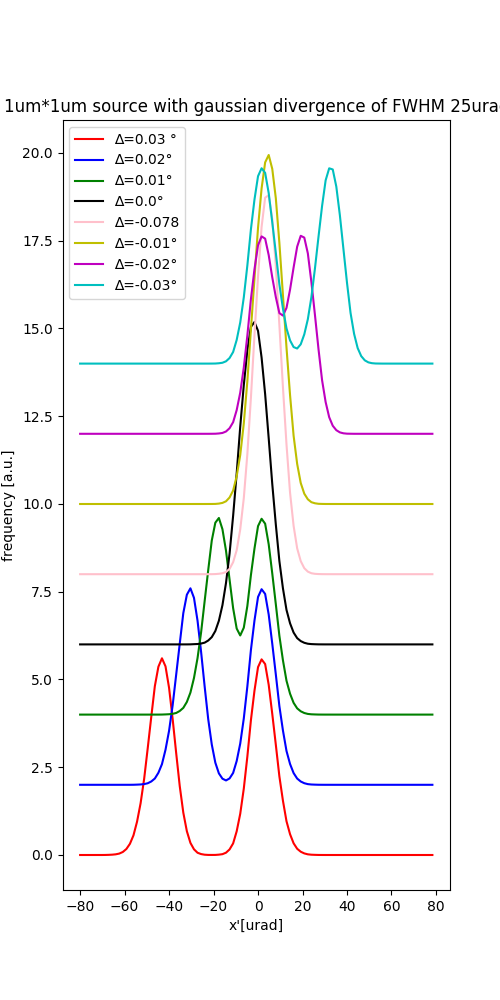
\includegraphics[width=0.8\textwidth]{histogram2.png}
\caption{\label{fig:histogram} x' values after the Montel system}
\end{figure}


\begin{figure}[H]
\centering
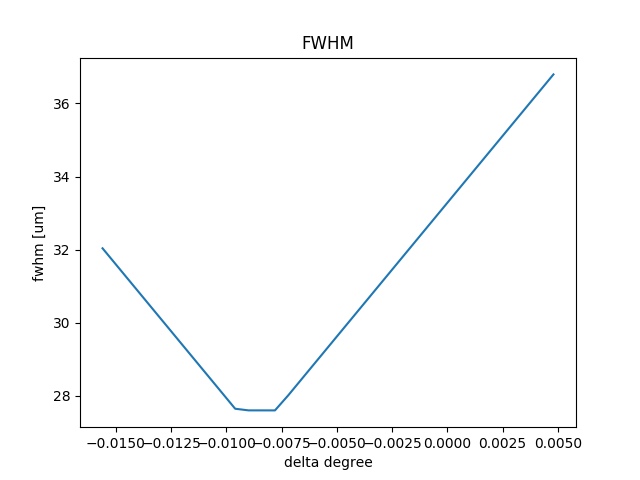
\includegraphics[width=0.8\textwidth]{FWHM.png}
\caption{\label{fig:FWHM} FWHM}
\end{figure}

\newpage
\appendix{Appendix A: how to find $\theta$}

\begin{figure}[H]
\centering
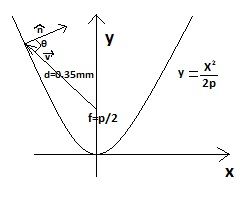
\includegraphics[width=0.6\textwidth]{pparabola_1_.jpg}
\end{figure}

\begin{equation*}
y=\frac{x^2}{2p}
\end{equation*}

\begin{equation*}
d=\sqrt[]{(x_p-x_0)^2+(y_p-y_0)^2}=\sqrt[]{x_p^2+(y_p-\frac{p}{2})^2}
\end{equation*}

\begin{equation*}
x_p=-0.0127046, y_p=0.350885
\end{equation*}

velocity to hit that point starting from $(0, \frac{p}{2})$
\begin{equation*}
v_x=-0.0363024, v_y=0.999341
\end{equation*}

normal at that point
\begin{equation*}
n_x=-0.984005, n_y=-0.17814
\end{equation*}

doing dot product between the normal and the velocity is possible to find
\begin{equation*} 
\theta=arcos(v_x*n_x+v_y*n_y)=88.962^\circ
\end{equation*}


\bibliographystyle{alpha}
\bibliography{sample}

\end{document}
